 \documentclass{beamer}

\usetheme{MagdeburgFIN}
\usefonttheme{structurebold}
\usepackage{graphicx}
\usepackage{wrapfig,lipsum}
\usepackage{float}
\usepackage{url}
\usepackage{pdfpages}
\usepackage[ngerman]{babel}
\usepackage[utf8]{inputenc}

\title{Database Operations on FPGAs}
\subtitle{Database Operations on FPGAs}
\author{Marten Wallewein-Eising}
\date{\today}
\institute{Otto von Guericke University, Magdeburg}

% Milestone II: Concept & additional literature research

\begin{document}

\begin{frame}[plain]
 \titlepage
\end{frame}

\section[Agenda]{}
\begin{frame}
	\frametitle{Agenda}
	\tableofcontents
\end{frame}

\section{Motivation and Introduction}
\begin{frame}
	\frametitle{Motivation}
	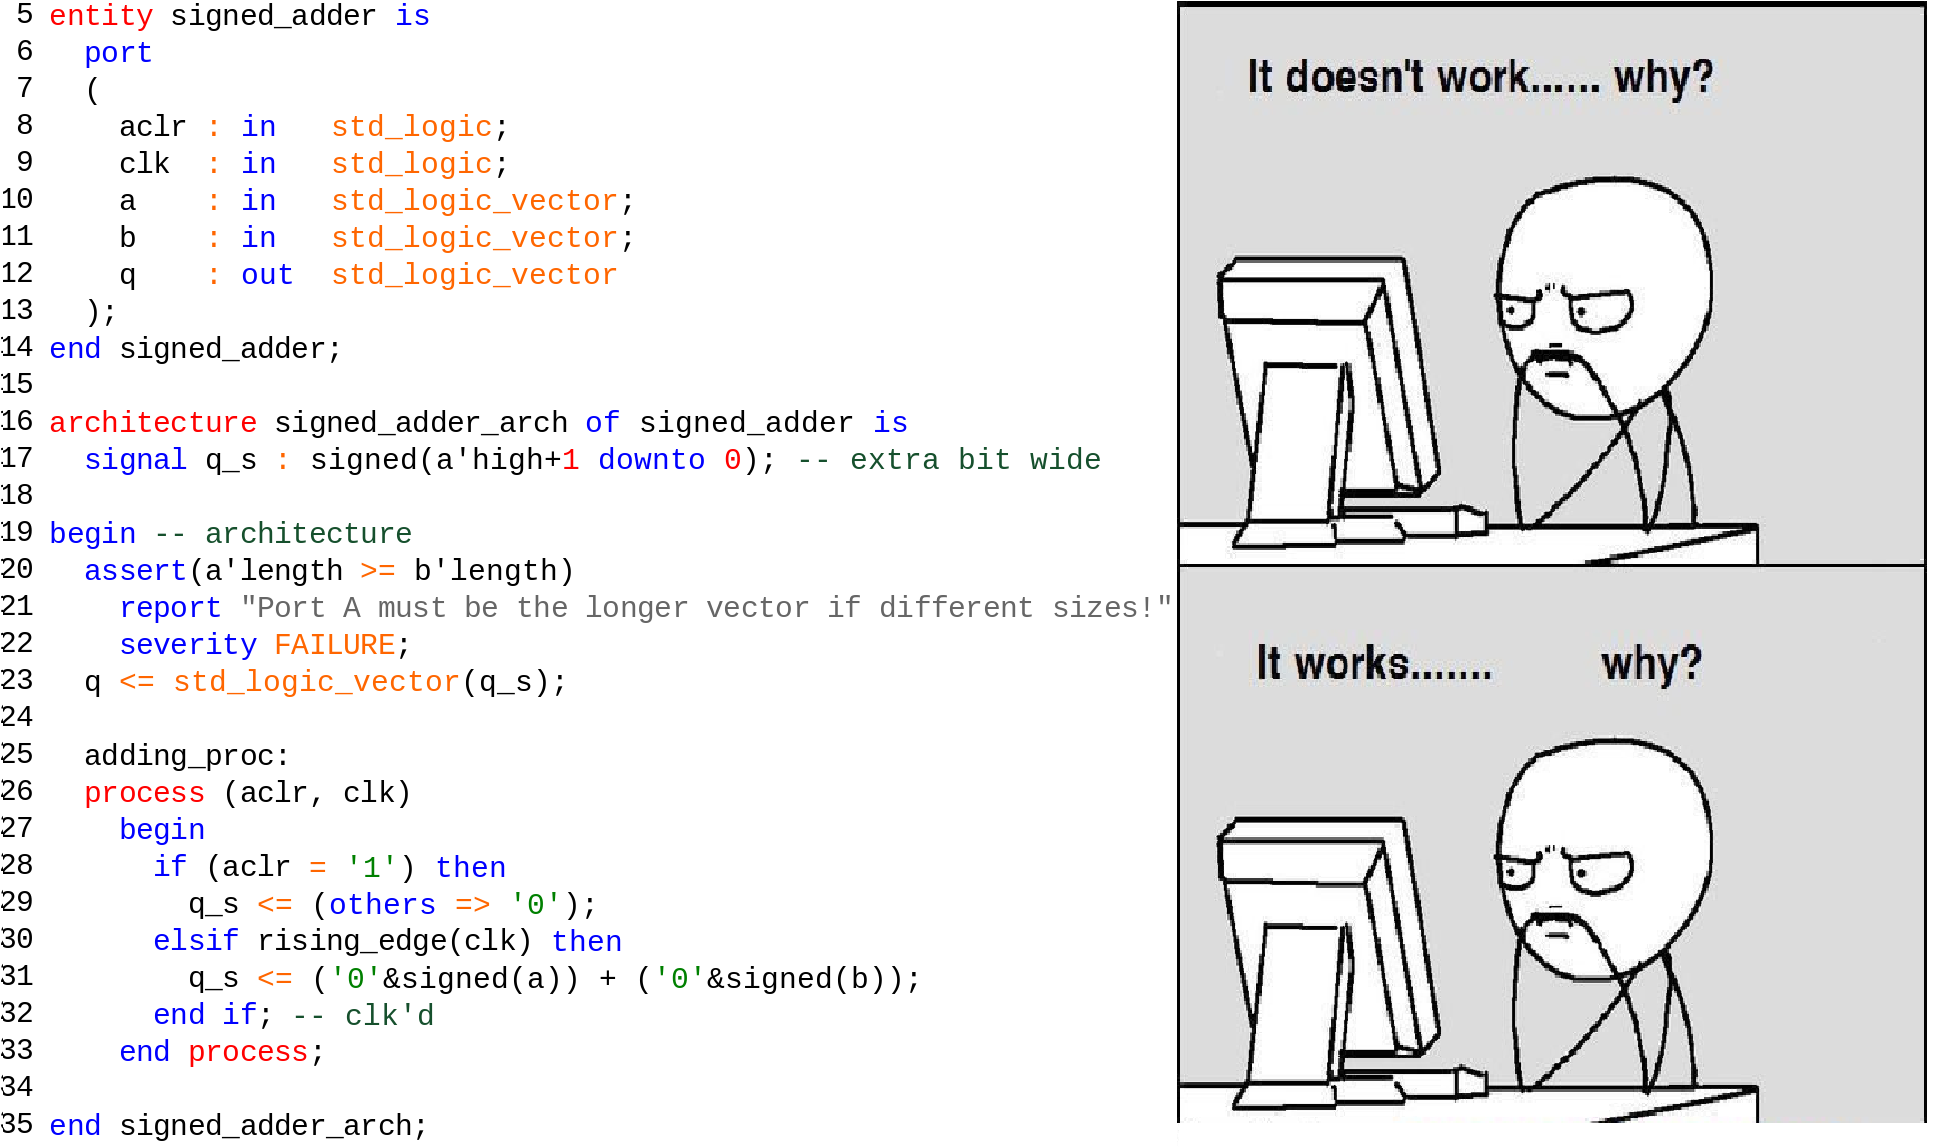
\includegraphics[width=1.0\textwidth]{img/complex_source.png}
	%\begin{itemize}
	%	\item Screen of complex HDL code?
	%	\item Why should we consider this stuff???
	%\end{itemize}
\end{frame}

\begin{frame}
	\frametitle{Problems with Moores Law}
	"Number of transistors in integrated circuit doubles about every two years"
	\vspace*{0.5cm}
	\begin{columns}
		\begin{column}{0.3\textwidth}
			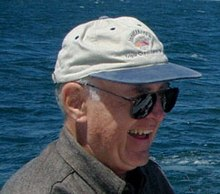
\includegraphics[width=1.0\textwidth]{img/gordon_moore.jpg}
			Gordon Moore
		\end{column}
		\begin{column}{0.66\textwidth}
				\begin{itemize}
				\item More transistors lead to more heat
				\item Not enough to increase cores and speed
				\item Memory/Power wall in von Neumann Architecture
				\item Fast growing data amounts (times 10 every 5 years)
				\item ...
			\end{itemize}
		\end{column}
	\end{columns}

\end{frame}

\begin{frame}
	\frametitle{Possible Solutions}
	Usage of different core types in CPU
	\begin{itemize}
		\item More variability, but cores must be generalized
	\end{itemize}
	\vspace*{0.5cm}%
	Usage of highly adapted Hardware (ASIC)
	\begin{itemize}
		\item High performance, but problem specific
	\end{itemize}
	\vspace*{0.5cm}%
	Usage of reconfigurable, programmable Hardware (FPGA)
	\begin{itemize} 
		\item Mix between generalization and performance
	\end{itemize}
	%\begin{itemize}
	%	\item Usage of different core types in CPU
	%	\item Usage of highly adapted Hardware (ASIC)
	%	\item Usage of reconfigurable, programmable Hardware => FPGA
	%	\end{itemize}
\end{frame}

\begin{frame}
	\frametitle{Introduction}
	\begin{center}
		\huge What is an FPGA?
	\end{center}
	
	"FPGAs consist of a plethora of uncommitted hardware resources, which can be
	programmed after manufacturing, i.e., in the field."
	%\begin{itemize}
	%	\item Field programmably gate array
	%	\item Questions?
	%\end{itemize}
	\vspace*{3cm}
	\begin{center}
		\small \emph{Data Processing on FPGAs}, Jens Teubner and Louis Woods 
	\end{center}
\end{frame}

\begin{frame}
	\frametitle{FPGA - Basics}
	\begin{itemize}
		\item Large resources of logic gates and RAM blocks to implement complex digital computations
		\item Designed to be configured after manufacturing
		\item Configuration is generally specified using a hardware description language (HDL)
		%\item Contains:
		%	\begin{itemize} 
		%		\item Array of programmable blocks
		%		\item Hierarchy of reconfigurable interconnects
		%	\end{itemize}
	\end{itemize}
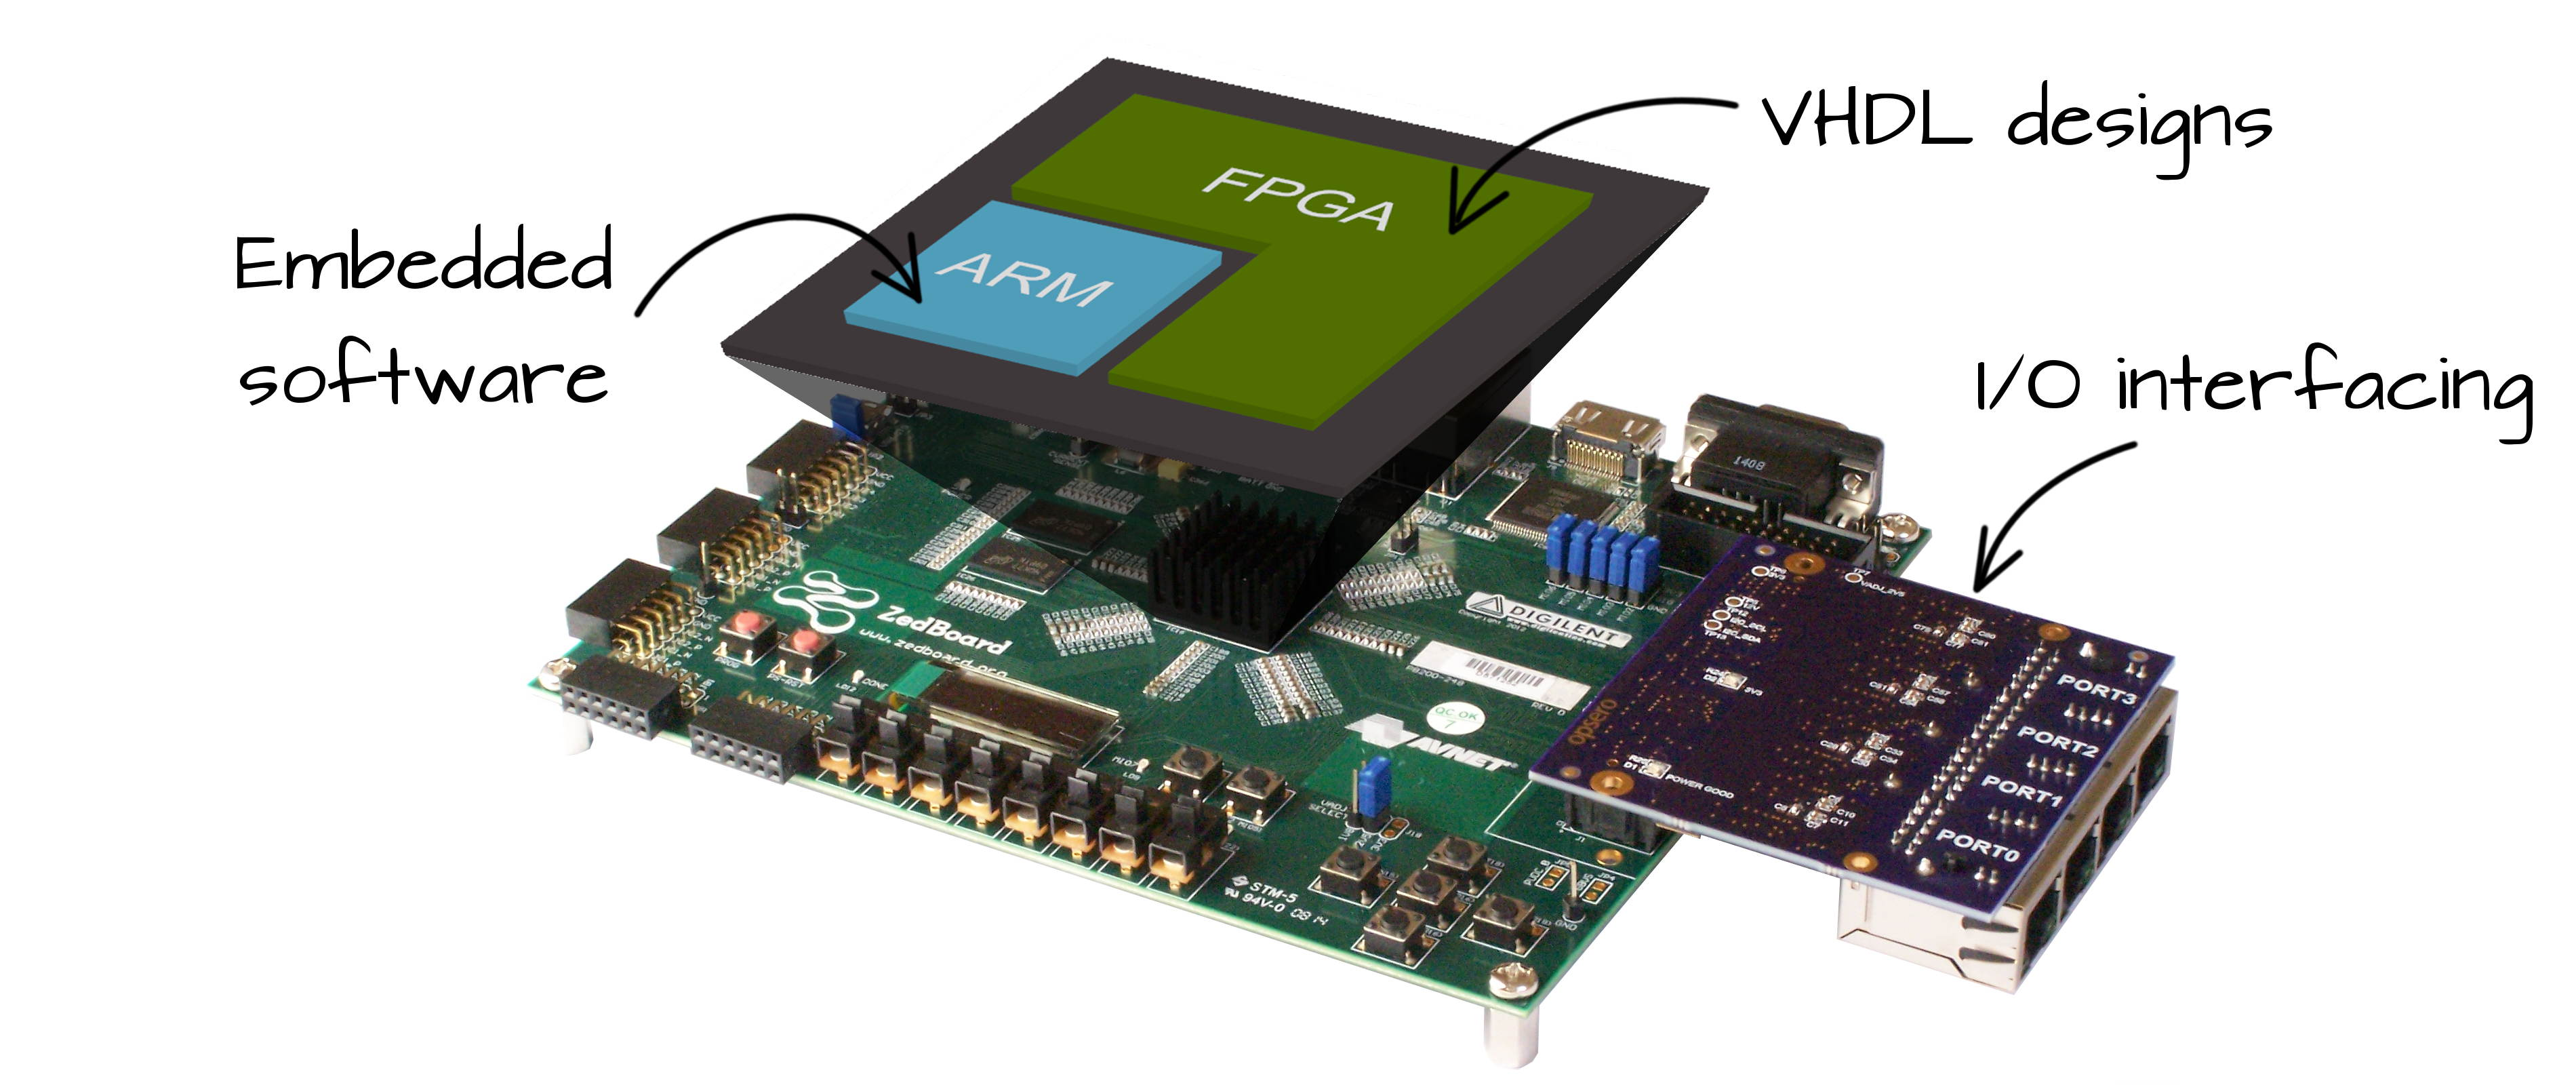
\includegraphics[width=1.0\textwidth]{img/fpga.jpg}
\end{frame}

\begin{frame}
	\frametitle{FPGA - Components}
	\begin{itemize}
		\item Lookup Tables: configurable type of logic gates
		\item Registers/Flip-Flops: Small storage types on chip
		\item BRAM: On Chip RAM storage
		\item DRAM: Off Chip RAM
		\item Hard cores: implementations of often-required functionality directly in silicon.
		\item Interconnect: wiring between all available ressources
	\end{itemize}
\end{frame}

\section{Benefits and Drawbacks}
\begin{frame}
	\frametitle{Benefits of FPGAs}
	\begin{itemize}
		\item Very low power consumption
		\item High flexibility in programming hardware components
		\item Dynamic reconfiguration at runtime
		\item High degree of data and instruction parallelism
	\end{itemize}
	\vspace*{0.3cm}
	\begin{center}
		"Custom hardware allows employing the most effective form of parallelization that best suits a given task."
	\end{center}
	\vspace*{0.1cm}
	\begin{center}
		\small \emph{Data Processing on FPGAs}, Jens Teubner and Louis Woods 
	\end{center}
\end{frame}

\begin{frame}
\frametitle{Drawbacks of FPGAs}
	\begin{itemize}
		\item Small amount of memory compared to high degree of parallelism
		\item High parallelism is very difficult to achieve
		\item Difficult and time consuming implementation of complex algorithms
		\item Bottleneck moves to data transfer to the FPGA 
	\end{itemize}
	\begin{center}
		"Building essentially a tailor-made piece of hardware takes the engineer beyond what he or she is used to in the software-only world."
	\end{center}
	\begin{center}
		\small \emph{FPGAs: A New Point in the Database Design Space}, Mueller et al.
	\end{center}
\end{frame}

\section{Integration in Database Systems}
\begin{frame}
	\frametitle{Integration in Database Systems}
	
	\textbf{How to integrate an FPGA into a Database System?}
	\begin{itemize}
		\item No complex operations due to small memory
		\item High IO throughput and degree of parallelism
		\item Difficult to implement and maintain various algorithms
	\end{itemize}
	\vspace*{1cm}
	\textbf{Conclusion: Basically, execute simple operations on huge data streams in parallel}
\end{frame}

\begin{frame}
\frametitle{Integration in Database Systems}
%Include graphic showing multiple integrations of FPGAs
\begin{center}
	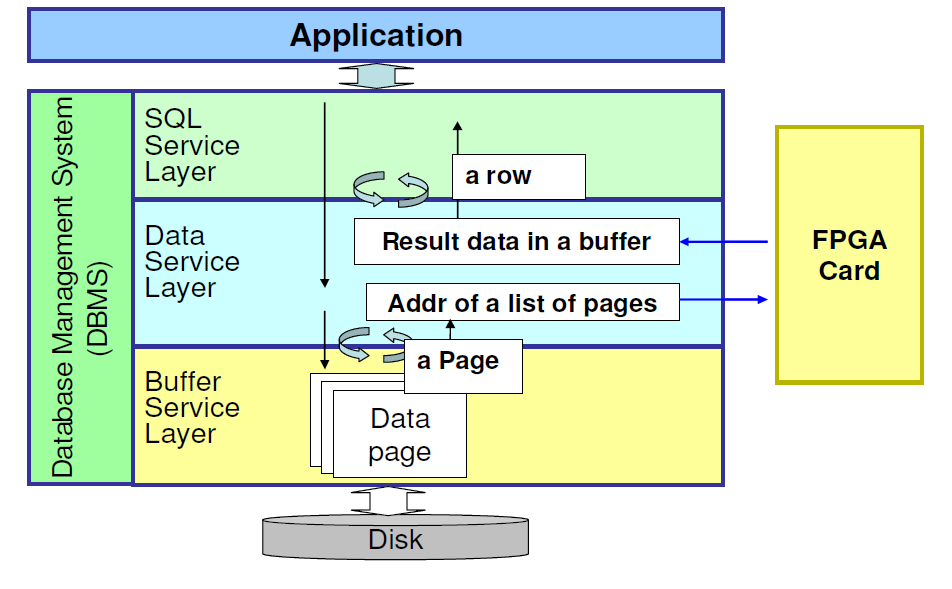
\includegraphics[width=0.9\textwidth]{img/integration.PNG}
\end{center}
\begin{center}
	\small \emph{Database Analytics Acceleration using FPGAs}, Sukhwani et al.
\end{center}
\end{frame}

\section{Database Operations}
\begin{frame}
	\begin{center}
		\huge Database Operations
	\end{center}
\end{frame}

\subsection{Co-Processing: Filter and Join Operations}
\begin{frame}
\frametitle{Filtering with FPGA Reconfiguration}
Energy aware SQL Query Acceleration:
\begin{itemize}
	\item Optimizer decides which parts are executed on FPGA
	\item Loading required modules for Query on Partial Area
	\item Tuples passed to FPGA and processed by modules
\end{itemize}
\vspace*{0.3cm}
Result:
\begin{itemize}
	\item Performance comparable to standard x86 systems
	\item 20 times higher energy-efficiency compared to MySQL
\end{itemize}
%\vspace*{2cm}
\begin{center}
	\small \emph{Energy-Aware SQL Query Acceleration through FPGA-Based Dynamic Partial Reconfiguration}, Becher et al.
\end{center}
\end{frame}

\begin{frame}
	\frametitle{Filtering with FPGA Reconfiguration}
	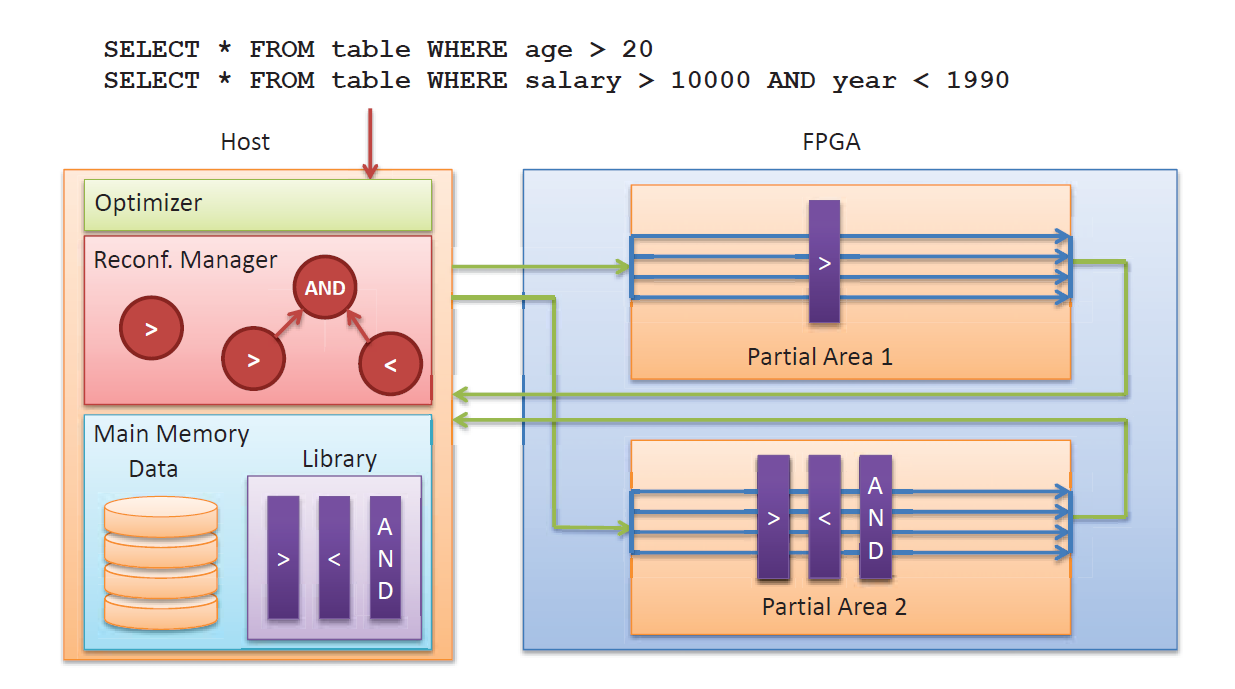
\includegraphics[width=0.9\textwidth]{img/reconf.png}
	\begin{center}
		\small \emph{Energy-Aware SQL Query Acceleration through FPGA-Based Dynamic Partial Reconfiguration}, Becher et al.
	\end{center}
\end{frame}

%\begin{frame}
%\frametitle{Sorting with MergeSort}
%\begin{itemize}
%	\item Due to high parallelism, a merge sorter can sort large datasets in short time
%	\item 
%	Koch and Torresen [2011] evaluated the FIFO merge sorter described above. Using 98\% of the available BRAM it was possible to sort 43,000 64-bit keys (344 KB) in a single iteration, i.e., by streaming the keys through the FPGA once. .e circuit could be clocked at MHz D fclk 252 resulting in a throughput of 2 GB/s.
%	\item Read: Data Processing on FPGAs
%\end{itemize}
%\end{frame}

\begin{frame}
	\frametitle{FPGA Framework for Join Operations}
	Processing hash-joins with a star scheme:
	\begin{itemize}
		\item Predicate evaluation and hash joining on FPGA as co-processor
		\item Equi-join queries with hash tables for efficient lookups
		\item 64Bit columns, FPGA running on 200Mhz 
	\end{itemize}
	Results:
	\begin{itemize}
		\item Speedup of 11.3 times compared to a 4.4Ghz multi-core system
	\end{itemize}
	\begin{center}
		\small \emph{Accelerating Join Operation for Relational Databases with FPGAs}, Halstead et al.
	\end{center}
\end{frame}

\begin{frame}
\frametitle{Summary: FPGA for Database Co-Processing}
Pro's:
\begin{itemize}
	\item High throughput and low power consumption
	\item Simple operations reach high parallelization
\end{itemize}
\vspace*{0.3cm}
Con's:
\begin{itemize}
	\item Bottleneck moves to data transfer to the FPGA
\end{itemize}
\vspace*{0.3cm}
\textbf{Conclusion:} For OLAP queries useful, OLTP query performance may suffer from data transfer time

\end{frame}

\subsection{Complete Query Execution}
\begin{frame}
	\frametitle{Complete Query Execution}
	\begin{center}
		\huge{Reconfiguration vs Frameworks}
	\end{center}
	
\end{frame}

\begin{frame}
	\frametitle{Query Execution - Reconfiguration}
	Glacier: Component Library and SQL to VHDL Compiler 
	\vspace*{0.2cm}
	\begin{columns}
		\begin{column}{0.48\textwidth}
			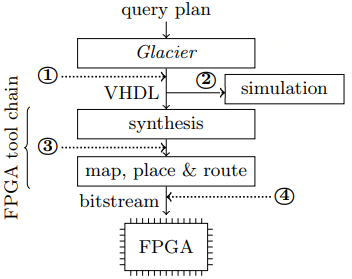
\includegraphics[width=1.0\textwidth]{img/glacier_2.png}
		\end{column}
		\begin{column}{0.48\textwidth}
			\begin{itemize}
				\item Translated to relational algebra tree, then compiled into hardware curcuits
				\item FPGA is reconfigured with the compilation result 
				\item Throughput rate guaranteed at compilation time
				%\item Draws its predictable runtime performance from statically allocating all hardware resources at circuit compilation time
			\end{itemize}
		\end{column}
	\end{columns}
\vspace*{0.2cm}
	\begin{center}
		\small \emph{Glacier: A Query-to-Hardware Compiler}, Mueller et al.
	\end{center}
\end{frame}

\begin{frame}
\frametitle{Query Execution - Reconfiguration}
\begin{center}
	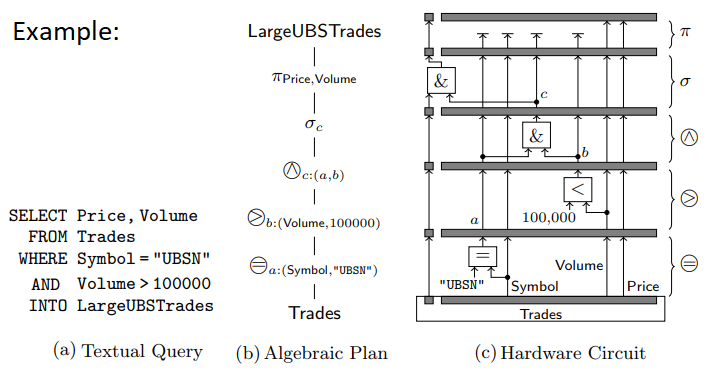
\includegraphics[width=1.0\textwidth]{img/glacier.png}
\end{center}
\begin{center}
	\small \emph{Glacier: A Query-to-Hardware Compiler}, Mueller et al.
\end{center}

\end{frame}

\begin{frame}
	\frametitle{Query Execution - Framework}
	FPGA based Acceleration Engine:
	\begin{itemize}
		\item Approach: Reconfiguration costs time
		\item Multiple generic Predicate Evaluation Units (PE)
		\item Each PE can evaluate a column of the row
	\end{itemize}
	\vspace*{0.2cm}
	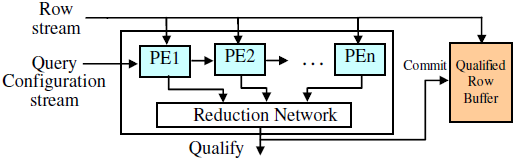
\includegraphics[width=0.9\textwidth]{img/row_stream.PNG}
	\vspace*{0.1cm}
	\begin{center}
		\small \emph{Database Analytics Acceleration using FPGAs, Sukhwani et al.}
	\end{center}
\end{frame}

\begin{frame}
	\frametitle{Query Execution - Framework}
	FPGA based Acceleration Engine:
	\begin{itemize}
		\item Benefits from extensive pipelining
		\item Use compression to fully load the pipeline
	\end{itemize}
	
	\begin{center}
		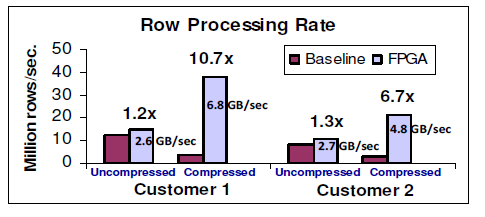
\includegraphics[width=0.8\textwidth]{img/engine_eval.png}
	\end{center}

	\begin{center}
		\small \emph{Database Analytics Acceleration using FPGAs, Sukhwani et al.}
	\end{center}
\end{frame}

\begin{frame}
\frametitle{Reconfiguration vs Frameworks?}
\begin{center}
	\begin{tabular}{| c | c | c |}
		\hline
		& Reconfiguration & Framework \\ \hline
		Pro's & Exact query matching & \\ \hline
		Con's & Reconfiguration time & \\ \hline
	\end{tabular}
\end{center}

\end{frame}

\section{Summary}
\begin{frame}
	\frametitle{Integrate an FPGA into a Database System?}
	\begin{itemize}
		\item Highly flexible use cases
		\item Reconfiguration vs Frameworks
		\item High throughput and low power consumption
		\item Very complicated to implement complex algorithms
		\item High potential in the future
	\end{itemize}
\end{frame}

\section{Sources}
\begin{frame}
	\frametitle{Sources - Literature}
	\begin{itemize}
		\item Mueller, Rene, Jens Teubner, and Gustavo Alonso. "Glacier: a query-to-hardware compiler." Proceedings of the 2010 ACM SIGMOD International Conference on Management of data. ACM, 2010.
		\item Becher, Andreas, et al. "Energy-aware SQL query acceleration through FPGA-based dynamic partial reconfiguration." Field Programmable Logic and Applications (FPL), 2014 24th International Conference on. IEEE, 2014.
		\item Halstead, Robert J., et al. "Accelerating join operation for relational databases with FPGAs." Field-Programmable Custom Computing Machines (FCCM), 2013 IEEE 21st Annual International Symposium on. IEEE, 2013.
	\end{itemize}
\end{frame}
\begin{frame}
\frametitle{Sources - Literature}
\begin{itemize}
	\item Teubner, Jens, and Louis Woods. "Data processing on FPGAs." Synthesis Lectures on Data Management 5.2 (2013): 1-118.
	\item Mueller, Rene, and Jens Teubner. "FPGAs: a new point in the database design space." Proceedings of the 13th International Conference on Extending Database Technology. ACM, 2010.
	\item Sukhwani, Bharat, et al. "Database analytics acceleration using FPGAs." Proceedings of the 21st international conference on Parallel architectures and compilation techniques. ACM, 2012.
\end{itemize}
\end{frame}

\begin{frame}
\frametitle{Sources - Images}
\begin{itemize}
	\item \url{https://wyncode.co/funniest-computer-programming-memes/}
	\item \url{https://upload.wikimedia.org/wikipedia/commons/thumb/6/6b/Gordon_Moore.jpg/220px-Gordon_Moore.jpg}
	\item \url{https://opsero.com/fpga-programming/}
\end{itemize}
\end{frame}
\begin{frame}
    \frametitle{Thank you for your attention!}
\end{frame}
\end{document}
